\documentclass[11pt]{article}
\usepackage[margin=1in]{geometry}
\usepackage{graphicx}
\begin{document}
\section*{R94 principal-open overlap bridge}
The frozen \texttt{overlap94-01} run checked seven named functions in
the accepted rank-32 source algebra. All 224 polynomial coordinates,
the full module products, both mapped overlap-unit identities, and
two corruption controls passed. A fresh S3 readback replay checked
all seven named vectors and the full matrix product.

\begin{center}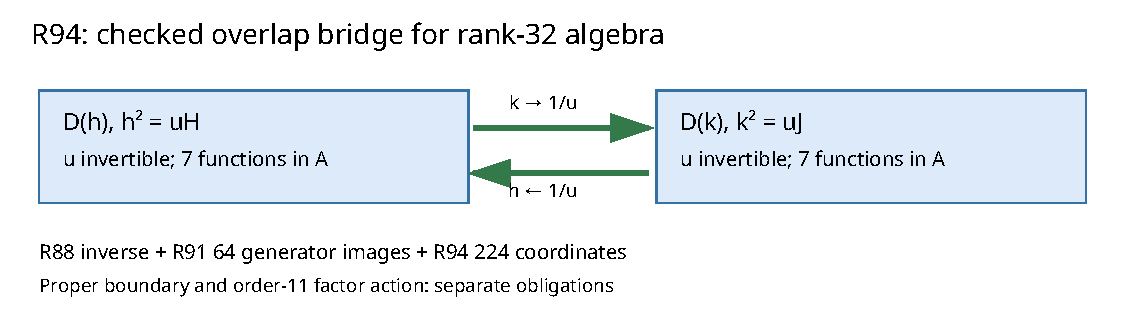
\includegraphics[width=.93\textwidth]{diagram.pdf}\end{center}

The identities $h^2=uH$ and $k^2=uJ$ make $u$ a unit on either principal
open. The chart maps send the opposite overlap unit to $1/u$.
Combined with R91 generator membership and R88 inverse composition,
this gives the overlap-ring bridge for the accepted rank-32 algebra.
The proper boundary identification and modular-factor action remain
separate checks. Source revision: \texttt{3c2ad242a}; raw archive
SHA-256: \texttt{79a58d0709cc09d4...fd56710ffc6dfccc}.
\end{document}
